\documentclass{automatisme}

\usepackage{tikz-repère}

\begin{document}

\begin{frame}
	\begin{minipage}{0.38\textwidth}
		\begin{center}
			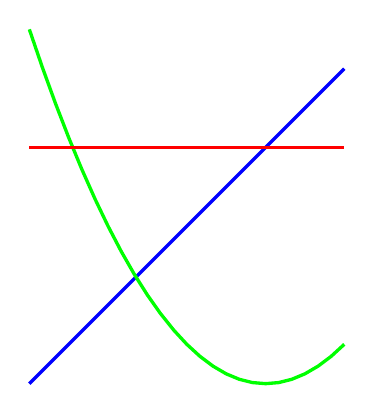
\begin{tikzpicture}[scale=0.5]
				\tikzRepere{-4}{4}{-2}{8}
				\draw<2->[domain=-4:4,very thick,blue] plot({\x},{\x + 3});
				\draw<2->[domain=-4:4,very thick,green] plot({\x},{0.25*\x*\x - \x});
				\draw<2->[domain=-4:4,very thick,red] plot({\x},{5});
			\end{tikzpicture}
		\end{center}
	\end{minipage}\hspace{0.05\textwidth}
	\begin{minipage}{0.52\textwidth}
		\begin{enumerate}
			\item Reproduire le repère ci-contre.
			\item Représenter dans ce repère les fonctions
			      \begin{itemize}
				      \setlength{\itemsep}{0.5em}
				      \item $f(x) = x - 3$
				      \item $g(x) = 0,25x² - x$
				      \item $h(x) = 5$
			      \end{itemize}
			\item Repérer graphiquement pour quelle(s) valeur(s) de $x$ on a :
			      \begin{itemize}
				      \setlength{\itemsep}{0.5em}
				      \item $f(x) = g(x)$
				      \item $g(x) = h(x)$
				      \item $f(x) = h(x)$
			      \end{itemize}
		\end{enumerate}
	\end{minipage}
\end{frame}

\begin{frame}
	\begin{center}
		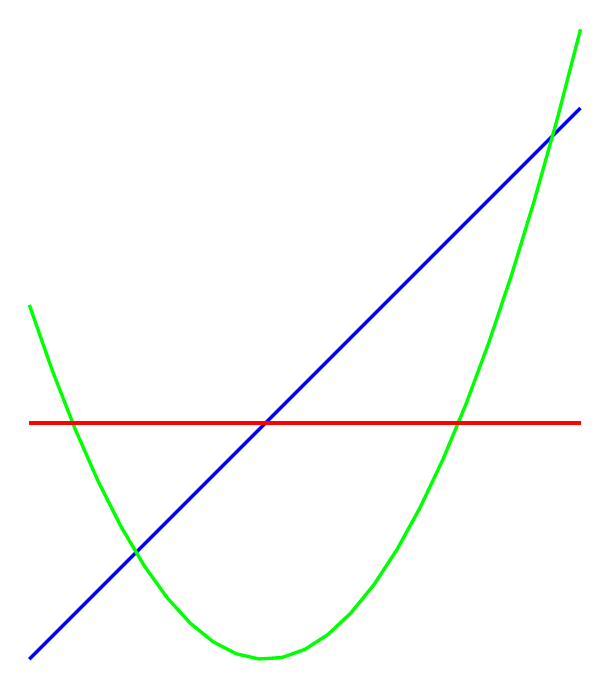
\begin{tikzpicture}[scale=0.5]
			\tikzRepere{-4}{10}{-2}{14}
			\draw[domain=-4:10,very thick,blue] plot({\x},{\x + 3});
			\draw[domain=-4:10,very thick,green] plot({\x},{0.25*\x*\x - \x});
			\draw[domain=-4:10,very thick,red] plot({\x},{5});
		\end{tikzpicture}
	\end{center}
\end{frame}

\end{document}